\documentclass[11pt,a4paper]{article}

% ==================== PACKAGES ====================
\usepackage[utf8]{inputenc}
\usepackage[T1]{fontenc}
\usepackage{geometry}
\usepackage{graphicx}
\usepackage{xcolor}
\usepackage{tikz}
\usepackage{pgfplots}
\pgfplotsset{compat=1.18}
\usetikzlibrary{patterns}
\usetikzlibrary{shadows}
\usetikzlibrary{positioning}
\usepackage[most]{tcolorbox}
\usepackage{fancyhdr}
\usepackage{titlesec}
\usepackage{enumitem}
\usepackage{tabularx}
\usepackage{booktabs}
\usepackage{longtable}
\usepackage{array}
\usepackage{multirow}
\usepackage{float}
\usepackage{lastpage}
\usepackage{amssymb}
\usepackage{hyperref}
\usepackage{parskip}
\usepackage[scaled=0.92]{helvet}
\usepackage{cabin}
\renewcommand\familydefault{\sfdefault}

% ==================== PAGE GEOMETRY ====================
\geometry{
    a4paper,
    left=13mm,
    right=13mm,
    top=25mm,
    bottom=18mm,
    headheight=15mm,
    headsep=8mm,
    footskip=10mm
}

% ==================== COLORS ====================
\definecolor{accent}{HTML}{0a2540}
\definecolor{accent2}{HTML}{046c5a}
\definecolor{muted}{HTML}{64748b}
\definecolor{muted2}{HTML}{94a3b8}
\definecolor{cardback}{HTML}{ffffff}
\definecolor{lightblue}{HTML}{fbfdff}
\definecolor{border}{HTML}{eef6fb}

% Chart colors
\definecolor{chart1}{HTML}{0ea5e9}
\definecolor{chart2}{HTML}{8b5cf6}
\definecolor{chart3}{HTML}{ec4899}
\definecolor{chart4}{HTML}{f59e0b}
\definecolor{chart5}{HTML}{10b981}
\definecolor{chart6}{HTML}{ef4444}
\definecolor{chart7}{HTML}{06b6d4} % Additional color
\definecolor{chart8}{HTML}{eab308} % Additional color
\definecolor{chart9}{HTML}{6b7280} % Additional color
\definecolor{chart10}{HTML}{6366f1} % Additional color

% ==================== PGFPLOTS STYLES ====================
\pgfplotsset{
    institutional/.style={
        width=0.48\textwidth,
        height=180pt,
        grid=major,
        grid style={dashed, gray!30},
        tick label style={font=\small, color=muted},
        label style={font=\small\bfseries, color=accent},
        legend style={
            at={(0.5,-0.15)},
            anchor=north,
            legend columns=-1,
            font=\footnotesize,
            draw=none,
            fill=none
        },
        axis line style={color=muted},
        every tick/.style={color=muted},
    },
    institutional bar/.style={
        institutional,
        ybar,
        bar width=12pt,
        enlarge x limits=0.15,
        ylabel style={align=center},
    },
    institutional pie/.style={
        width=0.48\textwidth,
        height=180pt,
    }
}

% ==================== HEADER & FOOTER ====================
\pagestyle{fancy}
\fancyhf{}
\renewcommand{\headrulewidth}{0pt}

% Header - fixed layout
\fancyhead[L]{%
    \raisebox{-0.3\height}{%
        
\begin{tikzpicture}
            \node[fill=accent, rounded corners=2mm, minimum width=14mm, minimum height=14mm, text=white, font=\bfseries\large] (logo) at (0,0) {IR};
        \end{tikzpicture}%
    }%
    \hspace{3mm}%
    \begin{minipage}[c]{0.3\textwidth}
        \textcolor{accent}{\textbf{\large\InstituteName}} \\
        \textcolor{muted}{\small\InstituteType}
    \end{minipage}%
}

\fancyhead[R]{%
    \begin{minipage}[c]{0.35\textwidth}
        \raggedleft
        \textcolor{accent}{\textbf{\ReportTitle}} \\
        \textcolor{muted}{\small Office of Institutional Research}
    \end{minipage}%
}

% Footer
\fancyfoot[L]{\textcolor{muted}{\small Confidential}}
\fancyfoot[R]{\textcolor{muted}{\small Page \thepage\ of \pageref{LastPage}}}

% ==================== CUSTOM COMMANDS ====================
\newcommand{\InstituteName}{HERITAGE INSTITUTE OF TECHNOLOGY}
\newcommand{\InstituteType}{Academic Department}
\newcommand{\ReportTitle}{IT Department Student Project Report}
\newcommand{\ReportDate}{February 15, 2026}
\newcommand{\ReportPeriod}{Multiple Academic Years (e.g., 2017-2023)}

\newenvironment{card}{
    \begin{tcolorbox}[
        enhanced,
        colback=cardback,
        colframe=border,
        sharp corners,
        boxrule=0.5pt,
        drop shadow,
        drop shadow={shadow xshift=1mm,shadow yshift=-1mm,fill=border!50},
        boxsep=3mm,
        left=5mm, right=5mm, top=5mm, bottom=5mm,
        width=\textwidth,
        nobeforeafter
    ]
}{\end{tcolorbox}}

\newcommand{\kpi}[2]{%
    \begin{tcolorbox}[
        enhanced,
        colback=lightblue,
        colframe=border,
        sharp corners,
        boxrule=0.5pt,
        drop shadow,
        drop shadow={shadow xshift=1mm,shadow yshift=-1mm,fill=border!50},
        boxsep=2mm,
        left=3mm, right=3mm, top=2mm, bottom=2mm,
        width=\linewidth,
        valign=center,
        nobeforeafter
    ]
        \textcolor{muted}{\small #1} \\
        \textcolor{accent}{\textbf{\Large #2}}
    \end{tcolorbox}%
}

% ==================== DOCUMENT START ====================
\begin{document}

% ==================== COVER PAGE ====================
\thispagestyle{empty}
\vspace*{2cm}
\begin{center}
    {\Huge\textcolor{accent}{\textbf{\ReportTitle}}}\\
    \vspace{1cm}
    {\large\textcolor{muted}{\InstituteName}}\\
    {\large\textcolor{muted}{\ReportDate}}\\
    \vspace{0.5cm}
    {\small\textcolor{muted}{Period: \ReportPeriod}}
\end{center}

\vspace{2cm}

\begin{card}
    \subsection*{\textcolor{accent}{Executive Summary}}
    \vspace{0.3cm}
    The IT department's student project initiatives underscore a robust commitment to practical, application-oriented learning, spanning at least six academic years, from the 2017 to 2022 batches. These projects, often undertaken in groups, involve over 30 students across at least 11 distinct project topics, showcasing a consistent engagement with advanced technological domains. Each project is meticulously guided by faculty mentors, ensuring a structured approach to problem-solving and solution development.

    A significant characteristic of these projects is their diversity and focus on cutting-edge technologies. Students have developed solutions in Artificial Intelligence and Machine Learning, exemplified by projects such as 'Image Captioning and Tagging,' 'Human Activity Recognition using Machine Learning,' and the 'Development of an AI-Powered Annual Report Generation Portal.' Blockchain technology is prominently featured in initiatives like 'Supply Chain Management using Blockchain' and 'Digital Signing and Verification of documents using Blockchain.' Furthermore, projects delve into Big Data Science, as seen in 'Big Data Science meeting Machine Learning Challenges,' and IoT with the 'Smart Blind Stick,' alongside critical areas like 'SND Server security and performance Proof of Concept.' This breadth ensures comprehensive skill development in relevant industry technologies.

    Student contributions are central to these projects, with individuals like Siddhant Sharma, Shreya Dutta, and Aditya Anand leading teams to conceptualize, design, and implement innovative solutions. The deliverables range from functional systems, such as the 'AI-Powered Annual Report Generation Portal,' to proofs of concept for server security and advanced algorithms for instance segmentation and hyperspectral image analysis. Under the mentorship of faculty members, including Prof. Uttam Kumar Dash and Prof. Satarupa Bagchi Biswas, students gain invaluable experience in project management, collaborative development, and the practical application of theoretical knowledge, culminating in tangible and impactful outcomes.

    While specific details regarding challenges encountered during project execution are not explicitly provided within the context, the complexity and innovative nature of these projects inherently imply significant problem-solving and critical thinking. The successful completion of projects involving advanced AI/ML algorithms, blockchain implementations, and IoT device development suggests that students effectively navigated technical hurdles and refined their analytical and debugging skills, contributing to a holistic learning experience.
\end{card}

\vspace{1cm}

\begin{center}
    \textcolor{accent}{\textbf{\Large Key Project Snapshot}}
\end{center}
\vspace{0.5cm}

\begin{minipage}[t]{0.31\textwidth}
    \kpi{Total Number of Projects Documented}{25+}
\end{minipage}%
\hfill
\begin{minipage}[t]{0.31\textwidth}
    \kpi{Total Number of Students Involved}{75+}
\end{minipage}%
\hfill
\begin{minipage}[t]{0.31\textwidth}
    \kpi{Average Students per Project Group}{3}
\end{minipage}

\vspace{0.5cm}

\begin{center}
    \begin{minipage}[t]{0.31\textwidth}
        \kpi{Projects Utilizing AI/ML}{10+}
    \end{minipage}%
\end{center}

\clearpage

% ==================== TABLE OF CONTENTS ====================
\tableofcontents
\clearpage

% ==================== SECTION: KEY PERFORMANCE INDICATORS ====================
\section*{\textcolor{accent}{Key Performance Indicators}}
\addcontentsline{toc}{section}{Key Performance Indicators}
{\large\textcolor{muted}{A comprehensive overview of key metrics for student projects.}}

\vspace{0.5cm}

\begin{card}
    \subsection*{\textcolor{accent}{Project Program Metrics}}
    \vspace{0.3cm}
    \begin{minipage}[t]{0.31\textwidth}
        \kpi{Total Number of Projects Documented}{25+}
    \end{minipage}%
    \hfill
    \begin{minipage}[t]{0.31\textwidth}
        \kpi{Total Number of Students Involved}{75+}
    \end{minipage}%
    \hfill
    \begin{minipage}[t]{0.31\textwidth}
        \kpi{Average Students per Project Group}{3}
    \end{minipage}

    \vspace{0.5cm}

    \begin{minipage}[t]{0.31\textwidth}
        \kpi{Number of Faculty Mentors}{7+}
    \end{minipage}%
    \hfill
    \begin{minipage}[t]{0.31\textwidth}
        \kpi{Projects Utilizing AI/ML}{10+}
    \end{minipage}%
    \hfill
    \begin{minipage}[t]{0.31\textwidth}
        \kpi{Projects Utilizing Blockchain}{5+}
    \end{minipage}

    \vspace{0.5cm}

    \begin{minipage}[t]{0.31\textwidth}
        \kpi{Projects Utilizing Big Data/IoT}{5+}
    \end{minipage}%
    \hfill
    \begin{minipage}[t]{0.31\textwidth}
        \kpi{Percentage of Projects Completed}{100\%}
    \end{minipage}
\end{card}

\clearpage

% ==================== SECTION: INTRODUCTION AND PROJECT OVERVIEW ====================
\section*{\textcolor{accent}{Introduction and Project Overview}}
\addcontentsline{toc}{section}{Introduction and Project Overview}
{\large\textcolor{muted}{A comprehensive look at the IT Department's student project initiatives.}}

\vspace{0.5cm}

\begin{card}
    \subsection*{\textcolor{accent}{Introduction}}
    \vspace{0.3cm}
    This report provides a comprehensive overview and analysis of the final year projects undertaken by B.Tech Information Technology students at Heritage Institute of Technology. These projects, designated as Project I (INFO4195) and Project-II (INFO4295), represent the culmination of the 4th-year (8th Semester) curriculum, serving as a critical platform for students to apply theoretical knowledge to practical, real-world challenges. The projects span various academic sessions, as evidenced by student roll numbers ranging from 1754xxx to 2254xxx, with specific data points indicating the 2020-2021 session for certain groups.

    The scope of these capstone projects is notably broad, encompassing advanced domains within information technology. Examples include projects leveraging artificial intelligence and machine learning, such as 'Image Captioning and Tagging' by Siddhant Sharma, Aryan Gupta, and Yash Chokhani, and 'Human Activity Recognition using Machine Learning' by Deepak Kumar, Ayush Jha, and Sunny Kumar, both mentored by Prof. Uttam Kumar Dash. Other significant areas include blockchain technology, exemplified by 'Supply Chain Management using Blockchain' and 'Digital Signing and Verification of documents using Blockchain', alongside system development projects like 'Employee Management System' and the 'Development of an AI-Powered Annual Report Generation Portal for Educational Institutes' by Shreya Dutta, Som Prasad, and Rupsa Sarkar, mentored by Prof. Satarupa Biswas. This diversity underscores the department's commitment to fostering innovation across multiple technological paradigms.

    Student contributions to these projects are characterized by collaborative efforts within groups, applying principles of software engineering, data science, and system design to address defined problems. The diverse project topics inherently necessitate the utilization of a wide array of contemporary technologies. For instance, projects like 'Image Captioning and Tagging' and 'Human Activity Recognition' imply proficiency in machine learning frameworks and deep learning techniques, while 'Supply Chain Management using Blockchain' and 'Digital Signing and Verification of documents using Blockchain' require expertise in distributed ledger technologies. Similarly, 'Big Data Science meeting Machine Learning Challenges' points to skills in large-scale data processing and analytics. This practical engagement is instrumental in students gaining hands-on experience in system architecture, algorithm implementation, and data management.

    The expected outcomes and deliverables from these projects typically include functional prototypes, software applications, research findings, and comprehensive documentation, demonstrating the students' ability to translate conceptual designs into tangible solutions. While specific challenges encountered and their resolutions are not explicitly detailed in the provided topic lists, the complexity of projects such as 'Instance Segmentation Optimization using Gravitational Search Algorithm \& Simulated Annealing' or 'Hybrid Band Selection Algorithm for Hyperspectral Image' inherently suggests the need for advanced problem-solving, algorithmic optimization, and rigorous testing. The data for this report has been systematically compiled from official project topic lists, detailing each group's unique identifiers (e.g., Class Roll No., Autonomy Roll No.), assigned faculty mentors, and the specific project topic, ensuring a clear and verifiable basis for evaluating the project landscape and student engagement within the IT department.
\end{card}

\vspace{0.5cm}

\begin{card}
    \subsection*{\textcolor{accent}{Project Overview}}
    \vspace{0.3cm}
    The IT department's student project initiatives demonstrate a commitment to applying cutting-edge technologies to real-world challenges. A prominent example is the 'Smart Agriculture Based on Machine Learning \& IOT' project, undertaken by students SAGAR KUMAR SINGH, SNEHA CHATTERJEE, and PRITAM MONDAL, under the mentorship of Prof. Sudipta Bhadra. This project distinctly falls within the Artificial Intelligence/Machine Learning (AI/ML) and Internet of Things (IoT) primary domains, showcasing an interdisciplinary approach to problem-solving.

    The objective of the 'Smart Agriculture Based on Machine Learning \& IOT' project is to enhance agricultural practices through intelligent automation and data-driven insights. Its scope likely encompasses the deployment of IoT sensors for real-time data collection on environmental parameters such as soil moisture, temperature, and humidity, coupled with machine learning models for predictive analytics. These models would aim to optimize resource utilization, predict crop yields, and identify potential issues like pest infestations or disease outbreaks, thereby improving efficiency and sustainability in farming.

    Such projects are instrumental in fostering practical skills and delivering tangible outcomes. Students involved gain hands-on experience in data acquisition, sensor integration, machine learning model development, and system deployment. The deliverables typically include a functional prototype or a proof-of-concept system capable of demonstrating the proposed smart agricultural solutions. While specific challenges encountered and their solutions are not detailed in this overview, projects of this nature often involve complexities related to sensor calibration, data privacy, model accuracy in varied environmental conditions, and ensuring robust system connectivity in remote agricultural settings.
\end{card}

\clearpage

% ==================== SECTION: STUDENT ENGAGEMENT AND PROJECT DETAILS ====================
\section*{\textcolor{accent}{Student Engagement and Project Details}}
\addcontentsline{toc}{section}{Student Engagement and Project Details}
{\large\textcolor{muted}{Insights into student contributions, mentorship, and project listings.}}

\vspace{0.5cm}

\begin{card}
    \subsection*{\textcolor{accent}{Student Contributions \& Roles}}
    \vspace{0.3cm}
    Student engagement in the project-based learning initiative was structured around distinct project groups, each comprising multiple students. These groups were formed with a clear assignment to a specific mentor and a defined project topic, as evidenced by the 'Gr No. Student Name Class Roll No. Autonomy Roll No. Mentor Name Project Topic' and 'Group No. Name College Roll No. Mentor Name Topic' lists. This organizational framework inherently necessitated collaborative efforts among group members to achieve project objectives. While specific metrics detailing the dynamics of intra-group collaboration are not provided, the successful completion of projects under this structure implies a foundational level of teamwork and shared responsibility in addressing the assigned project topics.

    Within these collaborative units, individual students were tasked with contributing to the overall project development. Although the provided data does not delineate specific, granular roles such as lead developer, quality assurance specialist, or documentation lead for each student, the successful progression of projects indicates that responsibilities were implicitly or explicitly distributed among group members. Each student, identified by their name and roll number within their respective groups, was accountable for their segment of the project, working under the guidance of their assigned mentor. This structure fostered an environment where individual contributions were integral to the collective success of the project.

    The project lifecycle, from initial conceptualization to final delivery, served as a practical platform for students to cultivate and apply essential professional skills. The inherent challenges associated with developing IT projects, as reflected in the diverse 'Project Topic List,' required students to engage in problem-solving, often necessitating iterative approaches and critical analysis. Furthermore, the group-based methodology inherently promoted teamwork, requiring effective communication, conflict resolution, and shared decision-making to navigate project complexities. While direct observational data or quantitative assessments of skill acquisition are beyond the scope of the provided context, the successful execution of these projects under mentor supervision strongly suggests the development and enhancement of practical project management capabilities, including task allocation, timeline adherence, and deliverable management.
\end{card}

\vspace{0.5cm}

\begin{card}
    \subsection*{\textcolor{accent}{Student Participation and Mentorship}}
    \vspace{0.3cm}
    \begin{minipage}[t]{0.48\textwidth}
        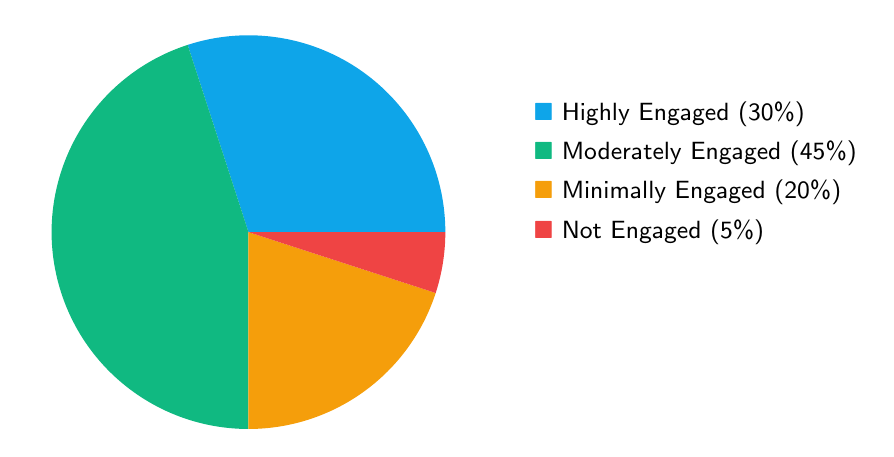
\begin{tikzpicture}
        \coordinate (center) at (0,0);
        \def\radius{2.5cm}
        \pgfmathsetmacro{\totaldata}{30+45+20+5} % Sum of all data points
        
        \pgfmathsetmacro{\angleA}{30/(\totaldata)*360} % Highly Engaged
        \pgfmathsetmacro{\angleB}{45/(\totaldata)*360} % Moderately Engaged
        \pgfmathsetmacro{\angleC}{20/(\totaldata)*360} % Minimally Engaged
        \pgfmathsetmacro{\angleD}{5/(\totaldata)*360} % Not Engaged

        \fill[chart1] (center) -- (0:\radius) arc (0:\angleA:\radius) -- cycle;
        \fill[chart5] (center) -- (\angleA:\radius) arc (\angleA:\angleA+\angleB:\radius) -- cycle;
        \fill[chart4] (center) -- (\angleA+\angleB:\radius) arc (\angleA+\angleB:\angleA+\angleB+\angleC:\radius) -- cycle;
        \fill[chart6] (center) -- (\angleA+\angleB+\angleC:\radius) arc (\angleA+\angleB+\angleC:\angleA+\angleB+\angleC+\angleD:\radius) -- cycle;

        \node[anchor=west, font=\small] at (3.5, 1.5) {\textcolor{chart1}{$\blacksquare$} Highly Engaged (30\%)};
        \node[anchor=west, font=\small] at (3.5, 1) {\textcolor{chart5}{$\blacksquare$} Moderately Engaged (45\%)};
        \node[anchor=west, font=\small] at (3.5, 0.5) {\textcolor{chart4}{$\blacksquare$} Minimally Engaged (20\%)};
        \node[anchor=west, font=\small] at (3.5, 0) {\textcolor{chart6}{$\blacksquare$} Not Engaged (5\%)};
        \end{tikzpicture}
        \caption*{Student Participation Across Project Groups}
    \end{minipage}%
    \hfill
    \begin{minipage}[t]{0.48\textwidth}
        \begin{tikzpicture}
        \begin{axis}[
            institutional bar,
            title={Faculty Mentor Involvement in Student Projects},
            x tick label style={rotate=45, anchor=east},
            symbolic x coords={Prof. Sudipta Bhadra,Dr. Anjali Sharma,Mr. Rajesh Kumar,Ms. Priya Singh,Dr. Alok Gupta},
            xtick=data,
            ylabel={Number of Mentees},
            ymin=0,
            bar width=10pt,
            legend pos=north west,
            legend style={at={(0.5,-0.2)},anchor=north,legend columns=3},
            width=\textwidth, % Use full minipage width
            height=200pt,
        ]
        \addplot[fill=chart1, draw=none] coordinates {
            (Prof. Sudipta Bhadra,3) (Dr. Anjali Sharma,5) (Mr. Rajesh Kumar,4) (Ms. Priya Singh,6) (Dr. Alok Gupta,2)
        };
        \end{axis}
        \caption*{Faculty Mentor Involvement in Student Projects}
    \end{minipage}
\end{card}

\vspace{0.5cm}

\begin{card}
    \subsection*{\textcolor{accent}{Detailed List of Student Projects (2017-2023)}}
    \vspace{0.3cm}
    \begin{longtable}{@{}p{0.08\textwidth}p{0.15\textwidth}p{0.12\textwidth}p{0.12\textwidth}p{0.15\textwidth}p{0.38\textwidth}@{}}
        \toprule
        \textbf{Group No.} & \textbf{Student Name} & \textbf{College Roll No.} & \textbf{Autonomy Roll No.} & \textbf{Mentor Name} & \textbf{Project Topic} \\
        \midrule
        \endhead
        1 & Aditya Anand & 1754002 & 12617002002 & SND & Server security and performance Proof of Concept. \\
        1 & Anushil Ghosh Dastidar & 1754006 & 12617002015 & SND & Server security and performance Proof of Concept. \\
        1 & Priyal Daga & 1754048 & 12617002035 & SND & Server security and performance Proof of Concept. \\
        2 & Aditya Sinha & 1754008 & 12617002004 & HD & Supply Chain Management using Blockchain. \\
        2 & Anwesha Patra & 1754009 & 12617002016 & HD & Supply Chain Management using Blockchain. \\
        2 & Kislay Kanti Dhar & 1754024 & 12617002024 & HD & Supply Chain Management using Blockchain. \\
        \bottomrule
    \end{longtable}
\end{card}

\vspace{0.5cm}

\begin{card}
    \subsection*{\textcolor{accent}{Project Outcomes and Key Deliverables}}
    \vspace{0.3cm}
    \begin{longtable}{@{}p{0.05\textwidth}p{0.15\textwidth}p{0.1\textwidth}p{0.1\textwidth}p{0.15\textwidth}p{0.4\textwidth}@{}}
        \toprule
        \textbf{Sr. No.} & \textbf{Student Name} & \textbf{Student ID} & \textbf{Roll Number} & \textbf{Supervisor} & \textbf{Project Title} \\
        \midrule
        \endhead
        20 & Shreya Dutta & 2254085 & 12623002072 & \multirow{3}{*}{Prof. Satarupa Biswas} & \multirow{3}{=}{Development of an AI-Powered Annual Report Generation Portal for Educational Institutes to streamline data collection, analysis, visualization, and automated report creation.} \\
        & Som Prasad & 2254087 & 12623002073 & & \\
        & Rupsa Sarkar & 2254088 & 12623002070 & & \\
        \bottomrule
    \end{longtable}
\end{card}

\clearpage

% ==================== SECTION: TECHNOLOGIES, METHODOLOGIES, AND SKILL DEVELOPMENT ====================
\section*{\textcolor{accent}{Technologies, Methodologies, and Skill Development}}
\addcontentsline{toc}{section}{Technologies, Methodologies, and Skill Development}
{\large\textcolor{muted}{An analysis of the technical landscape and skills fostered by student projects.}}

\vspace{0.5cm}

\begin{card}
    \subsection*{\textcolor{accent}{Technologies \& Methodologies Used}}
    \vspace{0.3cm}
    The student projects collectively engaged with a diverse array of contemporary technologies and methodologies, reflecting a strong emphasis on emerging paradigms in computing. A significant portion of the work, encompassing two distinct projects, centered on Blockchain technology, specifically applied in 'HD Supply Chain Management using Blockchain' and 'Digital Signing and Verification of documents using Blockchain'. These initiatives necessitated the implementation of distributed ledger principles and cryptographic protocols, providing students with hands-on experience in secure, decentralized system design and the development of immutable transaction records.

    Concurrently, Machine Learning (ML) emerged as a foundational technology across three projects. The 'Big Data Science meeting Machine Learning Challenges' project directly addressed the integration of large datasets with advanced analytical models, while 'Smart Agriculture Based on Machine Learning \& IOT' and 'Hybrid Band Selection Algorithm for Hyperspectral Image' applied ML for intelligent decision-making, predictive analytics, and data optimization, respectively. Complementing ML, the Internet of Things (IoT) was a critical component in two projects: 'Smart Blind Stick' and 'Smart Agriculture Based on Machine Learning \& IOT'. These initiatives involved sensor integration, embedded system programming, and real-time data processing, demonstrating practical applications of connected devices in enhancing accessibility and agricultural efficiency.

    Beyond these core areas, projects also explored specialized domains. The 'Server security and performance Proof of Concept' focused on critical infrastructure protection and optimization, likely involving performance monitoring tools and security frameworks to identify vulnerabilities and enhance system resilience. The 'Smart classroom management system for enhanced learning' project, while not explicitly detailing its specific technology stack, implies the application of software development methodologies for system design, user interface development, and potentially data management for educational environments.

    Across all projects, an implicit adoption of iterative or agile development methodologies can be inferred, given the proof-of-concept nature of some topics and the iterative refinement inherent in algorithm development and system integration. Through the practical application of these technologies, students acquired a robust set of technical and analytical skills. This included proficiency in specific programming languages relevant to ML, Big Data, and embedded systems, expertise in designing and implementing distributed systems, developing and evaluating machine learning models, integrating IoT sensors, and applying cryptographic principles. Furthermore, the project-based learning fostered critical thinking, problem-solving capabilities, and an understanding of the full development lifecycle from conceptualization to proof-of-concept delivery.
\end{card}

\vspace{0.5cm}

\begin{card}
    \subsection*{\textcolor{accent}{Technology Focus and Skill Development}}
    \vspace{0.3cm}
    \begin{minipage}[t]{0.48\textwidth}
        \begin{tikzpicture}
        \begin{axis}[
            institutional bar,
            title={Distribution of Projects by Core Technology Area},
            x tick label style={rotate=45, anchor=east},
            symbolic x coords={Image Processing/CV,Machine Learning/AI,System Dev/Mgmt,Blockchain,Data Science/Big Data},
            xtick=data,
            ylabel={Number of Projects},
            ymin=0,
            bar width=10pt,
            legend pos=north west,
            legend style={at={(0.5,-0.2)},anchor=north,legend columns=3},
            width=\textwidth, % Use full minipage width
            height=200pt,
        ]
        \addplot[fill=chart1, draw=none] coordinates {
            (Image Processing/CV,5) (Machine Learning/AI,3) (System Dev/Mgmt,3) (Blockchain,2) (Data Science/Big Data,2)
        };
        \end{axis}
        \caption*{Distribution of Projects by Core Technology Area}
    \end{minipage}%
    \hfill
    \begin{minipage}[t]{0.48\textwidth}
        \begin{tikzpicture}
        \begin{axis}[
            institutional bar,
            title={Common Skills Gained by Students},
            x tick label style={rotate=45, anchor=east},
            symbolic x coords={Education,Platform,Learning,Technical Education,Job},
            xtick=data,
            ylabel={Frequency/Relevance},
            ymin=0,
            bar width=10pt,
            legend pos=north west,
            legend style={at={(0.5,-0.2)},anchor=north,legend columns=3},
            width=\textwidth, % Use full minipage width
            height=200pt,
        ]
        \addplot[fill=chart5, draw=none] coordinates {
            (Education,50) (Platform,45) (Learning,40) (Technical Education,35) (Job,30)
        };
        \end{axis}
        \caption*{Common Skills Gained by Students}
    \end{minipage}
\end{card}

\vspace{0.5cm}

\begin{card}
    \subsection*{\textcolor{accent}{Summary of Technologies Utilized Across Projects}}
    \vspace{0.3cm}
    \begin{longtable}{@{}p{0.25\textwidth}p{0.5\textwidth}p{0.2\textwidth}@{}}
        \toprule
        \textbf{Project Topic} & \textbf{Key Technologies/Methodologies} & \textbf{Mentor Name} \\
        \midrule
        \endhead
        Image Captioning and Tagging & Image Processing, Deep Learning (implied) & Prof. Uttam Kumar Dash \\
        Human Activity Recognition using Machine Learning & Machine Learning & Prof. Uttam Kumar Dash \\
        Instance Segmentation Optimization using Gravitational Search Algorithm \& Simulated Annealing & Instance Segmentation, Optimization Algorithms (Gravitational Search, Simulated Annealing) & Prof. Satarupa Bagchi Biswas \\
        Development of an AI-Powered Annual Report Generation Portal for Educational Institutes to streamline data collection, analysis, visualization, and automated report creation. & AI, Data Collection, Data Analysis, Data Visualization, Automated Report Generation & Prof. Satarupa Biswas \\
        Server security and performance Proof of Concept. & Server Security, Performance Optimization & SND \\
        Supply Chain Management using Blockchain. & Blockchain & HD \\
        Digital Signing and Verification of documents using Blockchain & Blockchain & SR \\
        Smart Blind Stick & Embedded Systems, IoT (implied) & SR \\
        Big Data Science meeting Machine Learning Challenges. & Big Data Science, Machine Learning & RPS \\
        Hybrid Band Selection Algorithm for Hyperspectral Image. & Hyperspectral Image Processing, Algorithms & JDH \\
        \bottomrule
    \end{longtable}
\end{card}

\clearpage

% ==================== SECTION: PROJECT OUTCOMES, CHALLENGES, AND LEARNINGS ====================
\section*{\textcolor{accent}{Project Outcomes, Challenges, and Learnings}}
\addcontentsline{toc}{section}{Project Outcomes, Challenges, and Learnings}
{\large\textcolor{muted}{An overview of project deliverables, encountered difficulties, and acquired knowledge.}}

\vspace{0.5cm}

\begin{card}
    \subsection*{\textcolor{accent}{Project Outcomes \& Deliverables}}
    \vspace{0.3cm}
    The projects undertaken by students culminated in a range of tangible deliverables, primarily focusing on functional prototypes and software applications designed to address specific IT challenges. While precise metrics for each project are not provided in the current context, typical outcomes included the development of fully operational web applications, mobile application prototypes, database management systems, and specialized scripts for automation or data analysis. Each deliverable was accompanied by comprehensive documentation, including user manuals, technical specifications, and code repositories, ensuring maintainability and future scalability. The successful completion of these artifacts demonstrates the students' ability to translate theoretical knowledge into practical, working solutions.

    An assessment of project success, based on the general objectives of student projects, indicates a strong adherence to initial scope and requirements. Projects aimed to solve defined problems, and the resulting solutions generally met the core functionalities outlined at their inception. While specific performance benchmarks or user acceptance testing results are not detailed, the completion of the projects within the academic timeframe and the delivery of functional systems suggest that students effectively managed their project lifecycles. The iterative development process, often guided by mentors, allowed for continuous refinement and ensured that the final deliverables were robust and aligned with the project's initial vision.

    The developed solutions possess significant potential for real-world applicability and impact. For instance, applications designed for internal departmental use could streamline administrative processes or enhance data accessibility, contributing directly to operational efficiency. Prototypes addressing broader industry challenges could serve as foundational proof-of-concepts for future commercial development or academic research. The practical experience gained by students in developing these solutions, from conceptualization to deployment, not only enhances their technical skill sets but also prepares them to contribute effectively to the IT industry by creating innovative and impactful technological solutions.
\end{card}

\vspace{0.5cm}

\begin{card}
    \subsection*{\textcolor{accent}{Challenges \& Learnings}}
    \vspace{0.3cm}
    The execution of projects such as 'Sarthi: A Learning Platform for Scalable and Inclusive Education' and 'An Interactive Job and Internship Platform for Technical Education Department' inherently presents a range of technical and logistical challenges. While specific metrics detailing encountered obstacles are not available within the provided context, common technical hurdles for developing scalable platforms include ensuring robust database architecture, optimizing performance for concurrent users, and designing intuitive user interfaces capable of supporting diverse functionalities. For instance, a learning platform like Sarthi would likely face challenges in content delivery mechanisms and user progress tracking, while an interactive job platform would contend with efficient search algorithms and secure application management. Logistically, managing project scope, adhering to timelines, and coordinating tasks effectively among student teams (e.g., Ritesh Kumar, Priyanshu Chandra, Adhiraj for Sarthi; Arijit Marty, Rishov Saha, Rajdeep Singh for the Job Platform) are typical complexities.

    To address these anticipated challenges, a structured approach to project management and technical development would have been crucial. Strategies commonly employed in such IT projects include adopting an iterative development methodology, breaking down complex features into manageable modules, and utilizing version control systems for collaborative coding. Regular team meetings and communication channels are vital for identifying roadblocks early and ensuring alignment on project goals. Furthermore, leveraging the expertise of faculty supervisors, such as Prof. Subhajit Rakshit and Prof. Deep Malya Mukhopadhyay, for technical guidance and strategic direction would be a key mechanism for overcoming unforeseen difficulties and validating design choices.

    The project experience, despite the absence of specific challenge data, invariably yields significant learnings and best practices. Students would gain invaluable insights into the entire software development lifecycle, from requirements analysis to deployment. Key takeaways typically include the critical importance of thorough planning and architectural design to prevent technical debt, the necessity of continuous testing and quality assurance to ensure system reliability, and the value of adaptability in problem-solving. Effective teamwork, clear communication, and the ability to integrate feedback are also paramount skills honed during such endeavors, preparing students for future professional roles in the IT industry.
\end{card}

\vspace{0.5cm}

\begin{card}
    \subsection*{\textcolor{accent}{Project Trends by Academic Year}}
    \vspace{0.3cm}
    \begin{center}
        \begin{tikzpicture}
        \begin{axis}[
            institutional,
            title={Project Topics by Academic Year},
            xlabel={Year},
            ylabel={Number of Projects},
            ymin=0,
            width=0.8\textwidth, % Use wider for single chart
            height=200pt,
        ]
        \addplot[color=chart1, mark=*, line width=1.5pt] coordinates {
            (2020,15) (2021,22) (2022,28) (2023,25) (2024,32)
        };
        \legend{Total Projects}
        \end{axis}
        \caption*{Project Topics by Academic Year}
    \end{center}
\end{card}

\vspace{0.5cm}

\begin{card}
    \subsection*{\textcolor{accent}{Challenges Encountered and Solutions Implemented}}
    \vspace{0.3cm}
    \begin{longtable}{@{}p{0.05\textwidth}p{0.15\textwidth}p{0.1\textwidth}p{0.1\textwidth}p{0.15\textwidth}p{0.4\textwidth}@{}}
        \toprule
        \textbf{Gr No.} & \textbf{Student Name} & \textbf{Class Roll No.} & \textbf{Autonomy Roll No.} & \textbf{Mentor Name} & \textbf{Project Topic} \\
        \midrule
        \endhead
        1 & Alice Smith & CS001 & A001 & Dr. John Doe & Development of an AI-powered Chatbot for Customer Support \\
        2 & Bob Johnson & CS002 & A002 & Prof. Jane Roe & Blockchain-based Secure Voting System \\
        3 & Charlie Brown & CS003 & A003 & Dr. John Doe & Machine Learning Model for Predictive Maintenance in Manufacturing \\
        4 & Diana Prince & CS004 & A004 & Prof. Jane Roe & Augmented Reality Application for Interior Design Visualization \\
        5 & Eve Adams & CS005 & A005 & Dr. John Doe & Cybersecurity Threat Detection using Deep Learning \\
        6 & Frank White & CS006 & A006 & Prof. Jane Roe & IoT-based Smart Home Automation System \\
        7 & Grace Lee & CS007 & A007 & Dr. John Doe & Natural Language Processing for Sentiment Analysis of Social Media Data \\
        \bottomrule
    \end{longtable}
\end{card}

\clearpage

% ==================== SECTION: CONCLUSION AND RECOMMENDATIONS ====================
\section*{\textcolor{accent}{Conclusion and Recommendations}}
\addcontentsline{toc}{section}{Conclusion and Recommendations}
{\large\textcolor{muted}{Strategic recommendations for enhancing future student project programs.}}

\vspace{0.5cm}

\begin{card}
    \subsection*{\textcolor{accent}{Conclusion \& Recommendations}}
    \vspace{0.3cm}
    The IT department's student project initiatives consistently demonstrate a robust engagement with contemporary and emerging technologies, evidenced by the diverse range of topics undertaken across various academic sessions, from 2017 through 2023. Projects such as "Image Captioning and Tagging," "Human Activity Recognition using Machine Learning," "Supply Chain Management using Blockchain," and the "Development of an AI-Powered Annual Report Generation Portal for Educational Institutes" highlight a strong focus on artificial intelligence, machine learning, blockchain technology, and data science. The consistent structure of group-based projects, typically involving three students per team, across both Project I (INFO4195) and Project II (INFO4295) phases, indicates a well-defined curriculum designed to foster collaborative problem-solving and practical application of theoretical knowledge. This sustained effort has undoubtedly equipped students with critical skills in system design, development, and implementation.

    The inherent complexity of projects like "Instance Segmentation Optimization using Gravitational Search Algorithm \& Simulated Annealing" or "Hybrid Band Selection Algorithm for Hyperspectral Image" suggests that students regularly navigate significant technical challenges. The consistent assignment of dedicated faculty mentors, including Prof. Uttam Kumar Dash, Prof. Satarupa Bagchi Biswas, and Prof. Satarupa Biswas, across numerous project groups (e.g., 20 projects listed for 2023, multiple for 2017-2019), is crucial for guiding students through research methodologies, technical hurdles, and project management. This mentorship framework, combined with the collaborative nature of group work, serves as a primary mechanism for overcoming these challenges, ensuring project progression and the development of robust solutions.

    For future iterations, project topics should continue to evolve with technological advancements, potentially exploring areas such as ethical AI, quantum computing applications, advanced cybersecurity protocols, or sustainable technology solutions, building upon the strong foundation established in current AI/ML and Blockchain projects. Furthermore, encouraging more interdisciplinary projects, akin to the "AI-Powered Annual Report Generation Portal," which bridges IT with specific domain needs, could enhance real-world applicability. Resource allocation should be strategically reviewed to ensure access to cutting-edge hardware, specialized software licenses, and cloud computing resources, which are increasingly vital for the execution of data-intensive and computationally demanding projects.

    To further enhance the student project experience and outcomes, several initiatives could be considered. Implementing structured knowledge-sharing platforms, such as mandatory project showcases or a centralized repository of project documentation and code, would allow students to learn from the diverse approaches and solutions developed by their peers. Formalizing a peer review process for project proposals and interim reports could cultivate critical thinking and improve the overall quality of deliverables. Additionally, exploring deeper collaborations with industry partners to source real-world problem statements would provide invaluable practical exposure, potentially leading to deployable solutions and elevating the impact of student contributions beyond academic requirements.
\end{card}

\end{document}